
\documentclass[conference]{IEEEtran}
\IEEEoverridecommandlockouts
% The preceding line is only needed to identify funding in the first footnote. If that is unneeded, please comment it out.
\usepackage{cite}
\usepackage{amsmath,amssymb,amsfonts}
\usepackage{algorithmic}
\usepackage{graphicx}
\usepackage{textcomp}
\usepackage{xcolor}
\usepackage{enumitem}
\usepackage{cleveref}
\usepackage{array}
\def\BibTeX{{\rm B\kern-.05em{\sc i\kern-.025em b}\kern-.08em
    T\kern-.1667em\lower.7ex\hbox{E}\kern-.125emX}}
\begin{document}

\title{Adaptive and Generative
Music in Videogames\\

{\footnotesize \textsuperscript{}}
\thanks{}
}


\author{

\IEEEauthorblockN{Julius Emil Arendt}

\and
\IEEEauthorblockN{Jonas Pollpeter}
}

\maketitle

\begin{abstract}
Adaptive and generative music are
two techniques frequently used in
video games to create an immersive
audio environment. Adaptive music
involves changing the game's
soundtrack in response to the
player's actions, while generative
music uses algorithms to generate
unique compositions in real-time.
Both techniques offer game
developers a powerful tool to create
engaging and memorable gaming
experiences, and they are
constantly evolving with the latest
technological advancements.

Abstract dient als Zusammenfassung des Papers für den Leser und sollte daher als letztes geschrieben werden.
\end{abstract}

\section{Introduction}
The aim of this paper is to summarise current developments and research on adaptive and generative music in video games. Firstly, the two different forms of adaptive and generative music are introduced. This is followed by an explanation of some current systems and techniques for implementing adaptive and generative music. Then the techniques presented are compared and the advantages and disadvantages are discussed. This discussion is particularly focused on the effects and the impact on the player. Finally, technical challenges, problems and limitations are mentioned. 

\subsection{Music in Video Games}
Music has an important effect in video games \cite{fu2015backgroundmusic}. Most video games use music to emphasize specific emotions and improve the tension and immersion. For this purpose linear music is used by the majority of video games \cite{prechtl2016adaptive}. Linear music is static and does not change in relation to the interaction of the player. But the video game itself is often not linear and reacts dynamically to player interactions. This can cause a conflict between the static audio and dynamic visual response of a video game, as the music may not fit perfectly to every state of the game \cite{plut2022preglam}.

Due to hardware limitations, older video games such as Super Maio Bros from 1985 \cite{supermariobros1985} mostly use linear music \cite{plut2020generative}. However, advances in hardware have made it possible for current video games to implement customized music. This customized music can be grouped in adaptive and generative music \cite{plut2020generative}. In contrast to linear music, adaptive and generative music react to the player's interactions during the runtime of the video game \cite{plut2020generative}. This allows the music to be better adapted to the current game state.

\subsection{Adaptive Music}
Adaptive music, also referred to as interactive music, features a dynamic composition of different music fragments \cite{plut2020generative} \cite{hutMcCormAms} \cite{amaral2022adaptive}.
The composition can be organized using information about the game, such as variables or game states \cite{plut2020generative}. 
Furthermore, the composition of the music can also be changed on different levels such as tempo, pitch, volume \cite{plut2020generative} \cite{amaral2022adaptive}.

\subsection{Generative Music}
Generative music is sometimes also referred to as procedural or algorithmic music \cite{plut2020generative}. As the name suggests, generative music creates new music at runtime \cite{amaral2022adaptive}. The generation can be based on algorithms, rules or specific models \cite{plut2020generative} \cite{amaral2022adaptive}. 

Plut et al. group different types of generative music into two categories: academic and industry applications \cite{plut2022preglam}. They describe how the academic approach usually tries to replace explicitly composed pieces of music with generated music \cite{plut2022preglam}. The creation of the music is usually based on affective models that attempt to depict the various emotions of the player \cite{plut2022preglam}. In contrast, the industry approach to generative music often uses explicitly composed pieces of music that are extended in real time using generative music systems \cite{plut2022preglam}. These generative systems can, for example, use stochastic processes to combine different music fragments in new ways depending on game variables \cite{plut2022preglam}.

\subsection{Discussion}
The discussion and comparison of the various techniques centres on the effect and impact on the player. Particular attention is paid to whether the systems improve immersion and the gaming experience compared to linear music. Furthermore, it is discussed how reliable these systems are and whether linear music might achieve better results in some cases.
\section{Adaptive Music System (Julius)}

In the year 2019, the authors Patrick Hutchings and Jon McCormack
introduced the Adaptive Music System (AMS) \cite{hutMcCormAms} 
and tested it with several evaluators. It was developed as a
stand-alone package that receives game information from the
video game itself in real-time to generate a model of the game-
state and output music from this state \cite{hutMcCormAms}. Their
system is divided into two main components: 
\begin{enumerate}[label=\arabic*)]
    \item A spreading activation model to read the game's information \cite{hutMcCormAms}.
    \item The music generation system that uses the spreading activation model output to generate its music \cite{hutMcCormAms}. 
\end{enumerate}

\subsection{Spreading Activation model}



\section{Generative Music System based on Deep Learning Transformer Model (Julius)}

Hier wird die Architektur basierend auf dem Deep Learning Transformer Model vorgestellt.

\section{PreGLAM and Multitrack Music Machine}

\subsection{PreGLAM}

The Predictive Gameplay-based Layered Affect model (or short: PreGLAM)
was developed to be integrated flexibly into the design process of a 
game \cite{plut2023preglam}. PreGLAM is an artificial cognitive agent
designed to replicate the real-time emotional perceptions of a biased 
game spectator \cite{plut2023preglam}. PreGLAM calculates an estimation
of the game spectator's perceived emotion, which is based on the 
events in the game and other variables \cite{plut2023preglam}.

The PreGLAM models a spectator who has a certain game outcome as
a desire, but PreGLAM itself is not capable of affecting the gameworld
\cite{plut2023preglam}. The authors of PreGLAM modeled with the desire
of the player winning the game, but they also state that there could 
be any quantifiable outcome used \cite{plut2023preglam}.

\subsubsection{Architecture}

\begin{figure}[h]
    \centering
    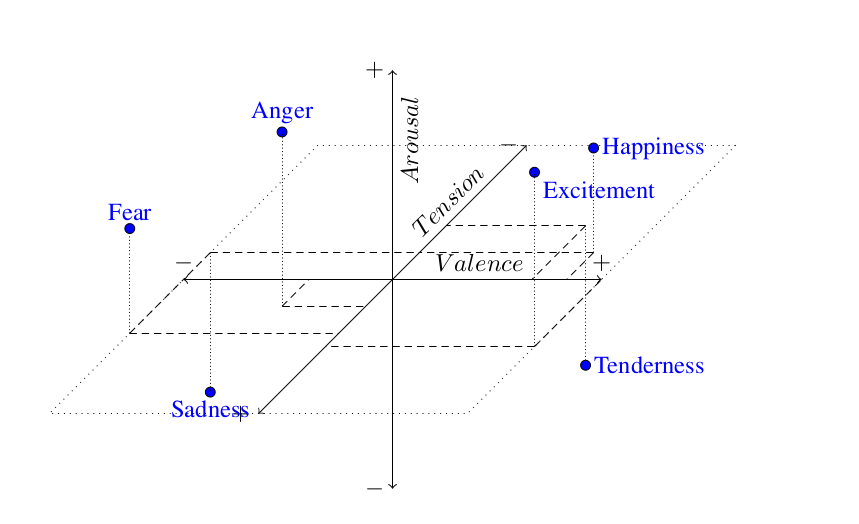
\includegraphics[width=\linewidth]{images/vat_model.png}
    \caption{3-Dimensional VAT Model of Affect, with example emotion categories placed for reference \cite{plut2023preglam}}
    \label{fig:vat_model}
\end{figure}

PreGLAM uses VAT model of affect \cite{plut2023preglam}. It has the dimensions
Valence, Arousal and Tension, as you can see in \Cref{fig:vat_model}. 

The authors describe Valence as a description of the current mood, whether it
is positive or negative \cite{plut2023preglam}. For instance, if a racing
game is played, and the own car passes another car which increases
the own car's position, or the own car crashes another car, the affect might be 
positive \cite{plut2023preglam}.
Nevertheless, getting hit by a car or being passed by someone else could 
possibly decrease the Valence value \cite{plut2023preglam}.

The Arousal in this context sometimes is paraphrased as "activity" or "energy", 
simulates the activation, or the intensity of an emotion \cite{plut2023preglam}.
High arousal emotions are emotions like excitement and fear, low arousal emotions
are emotions like calmness and sadness \cite{plut2023preglam}. 

\begin{figure}[h]
    \centering
    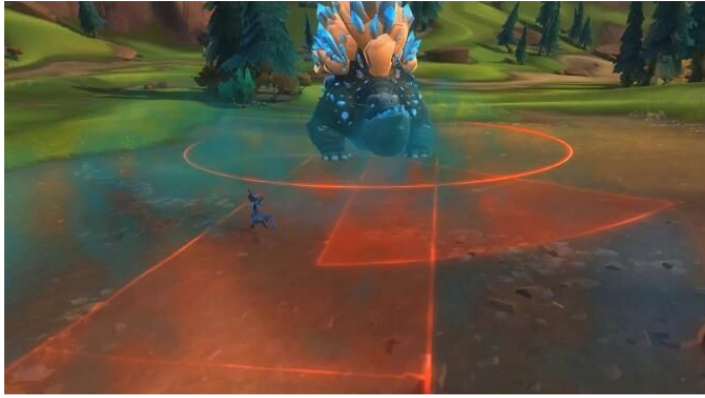
\includegraphics[width=\linewidth,height=4cm]{images/wildstar_attack_indicator.png}
    \caption{Attack telegraphs from Wildstar \cite{nixius2014wildstartelegraph}. The red areas indicate that an attack is coming soon (Figure and caption from \cite{plut2023preglam})}
    \label{fig:wildstar_indicator}
\end{figure}

The Tension involves the prospect or prediction of a future event
\cite{plut2023preglam}. It may be high if the next event might
be positive, but also negative in the case of a negative event
\cite{plut2023preglam}. An example of a future event can be seen
in \Cref{fig:wildstar_indicator}. It shows a set of attack telegraphs
from the MMO wildstar \cite{nixius2014wildstartelegraph} which 
communicate an event of incoming attack to the 
player\cite{plut2023preglam}. This may increase the tension, which
can lead the player to prevent or dodge the incoming attack 
\cite{plut2023preglam}.

Next to the gameplay desire the player can have, PreGLAM
also takes a set of events as input, which are annotated based
on how they affect the given desire, how strong their effect
on the desire is, and the values of variables which provide the 
gameplay context \cite{plut2023preglam}.

PreGLAM overlays its event-focused emotion rating model with an ambient mood score to generate a single affect score per dimension every 250 ms \cite{plut2023preglam}. PreGLAM calculates an emotion score from both events that have already occurred and predicted events \cite{plut2023preglam}. In addition, PreGLAM scales the emotion scores over time to reflect the ebb and flow of emotions over time \cite{plut2023preglam}.



\subsection{Multi-Track Music Machine}

\begin{figure}[h]
    \centering
    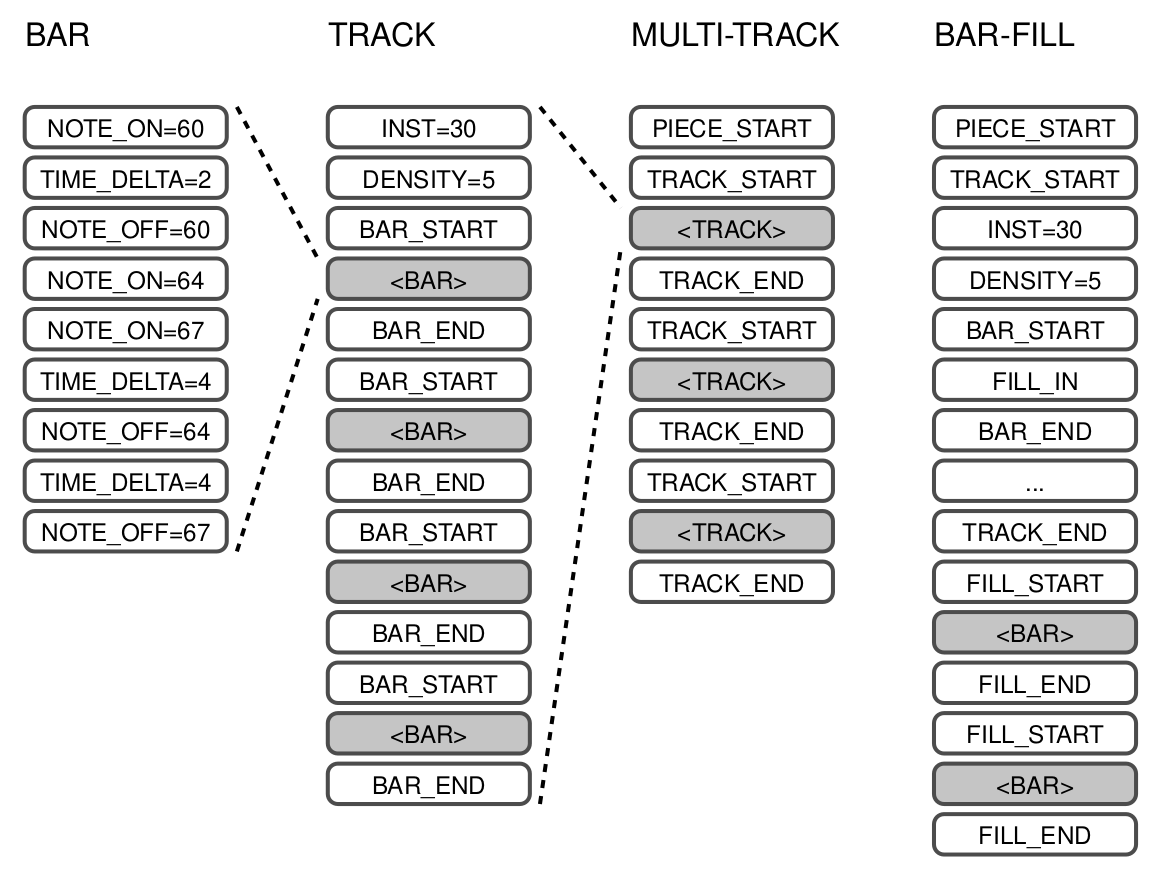
\includegraphics[width=\linewidth]{images/bar_fill_multi_track.png}
    \caption{The MultiTrack and BarFill representations are shown. The BAR tokens cor-
respond to complete bars, and the TRACK tokens correspond to complete tracks. (Figure and caption from \cite{ens2020mmm})}
    \label{fig:multi_track_figure}
\end{figure}

The Multi-Track Music Machine (MMM) was developed by Jeff Ens and Philippe Pasquier and is a generative music system that uses the Transformer architecture \cite{vaswani2017transformer} and is able to generate multi-track-music \cite{ens2020mmm}.

\subsubsection{Architecture and MultiTrack representation}

The representation of Tracks, Multi-Tracks, Bars and the Bar-Fill can be seen in \Cref{fig:multi_track_figure}.
The Bar representation consists of 128 NOTE\_ON tokens, 128 NOTE\_OFF tokens and 
48 TIME\_SHIFT tokens \cite{ens2020mmm}. The authors state
that due to the fact that musical events are quantised using 12 subdivisions per beat, the 48 used TIME\_SHIFT tokens
can be used for any rhytmic unit from
sixteenth note triplets to a full 4-beat
bar of silence \cite{ens2020mmm}. A bar 
starts with a BAR\_START token and ends
with a BAR\_END token \cite{ens2020mmm}. 

Tracks in this representation contain a sequence of bars and start with a 
TRACK\_START token and end with a TRACK\_END token \cite{ens2020mmm}.
After the TRACK\_START token, the track itself begins with the INSTRUMENT token \cite{ens2020mmm}.
It is used to specify the MIDI program that is used to play the notes on a 
certain track \cite{ens2020mmm}. There are 128 different INSTRUMENT tokens \cite{ens2020mmm}.
After the INSTRUMENT token follows the DENSITY\_LEVEL token, which specifies the note 
density of the track that is currently played \cite{ens2020mmm}.

A piece consists of multiple tracks and begins with a PIECE\_START token,
where bars are put into tracks, and tracks are put into a piece \cite{ens2020mmm}.
A PIECE\_END token is not used within a piece, because a piece contains exactly 
n tracks \cite{ens2020mmm}.

With the help of the MultiTrack representation, the model learns to make the generation
of every track dependent of of the pre-generated track \cite{ens2020mmm}.
During the generation, the process allows for a subset of the musical material to be
fixed while generating additional tracks \cite{ens2020mmm}.

Nevertheless, the MultiTrack representation introduced by Ens and Pasquier only offer control at the track level, but not at the bar level, except the model is asked to complete the remaining bars of a track \cite{ens2020mmm}. In order to achieve this, 
the authors remove all the bars to be predicted and replace each of them with a
FILL\_PLACEHOLDER token \cite{ens2020mmm}. 

After the removal, the removed bars are inserted at the end of a track, more specifically,
after the last TRACK\_END token \cite{ens2020mmm}. As the bars get inserted in the same 
order they got removed, they get wrapped with FILL\_START and FILL\_END tokens instead of 
BAR\_START and BAR\_END token \cite{ens2020mmm}. The authors call the resulting 
representation the BarFill representation \cite{ens2020mmm}.

\subsubsection{Training of MMM}

The authors use the Lakh MIDI Dataset \cite{raffel2016learning} for training their system \cite{ens2020mmm}. According to the authors, the training is done on a GPT2 model from 
Radford et al. \cite{radford2019language}, together with the HuggingFace Transformers
library of Wolf et al. \cite{wolf2019huggingface} using 8 attention heads, 6 layers, an
embedding size of 512 and an attention window of 2048 \cite{ens2020mmm}.

\subsection{PreGLAM-MMM}

For evaluation purposes, the authors of \cite{plut2022preglam} used the PreGLAM
emotion model \cite{plut2023preglam} and the Multi-Track Music 
Machine \cite{ens2020mmm} in their own game called Galactic Defense \cite{plut2022preglam}.


Galactic Defense is an action-RPG game, in which the player utilizes a set of
abilities, which are used to defeat a set of enemy units 
utilizing a recharging but limited resource pool, where he has 
to take care to not use certain abilities while beeing attacked \cite{plut2022preglam}.

\begin{figure}[h]
    \centering
    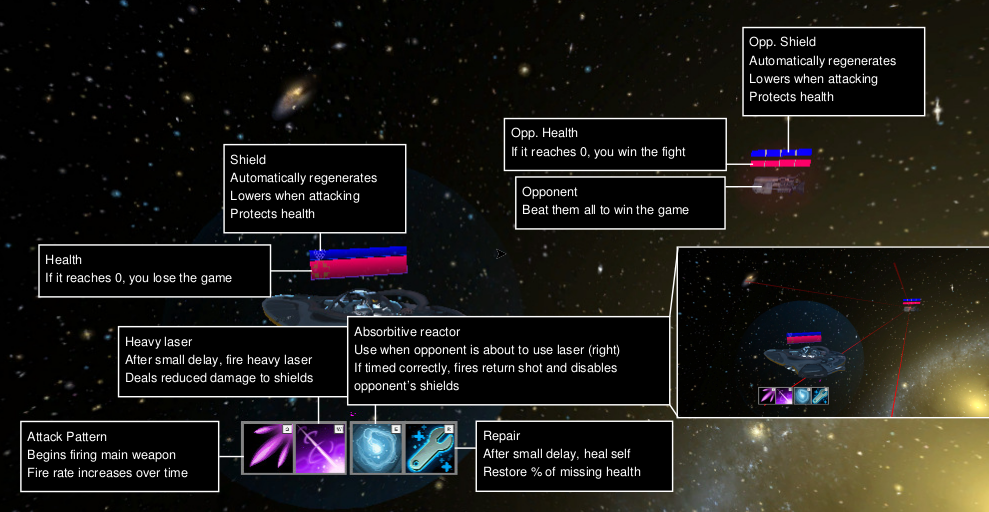
\includegraphics[width=\linewidth]{images/tutorial_gal_def.png}
    \caption{Tutorial scene of Galactic Defense \cite{plut2022preglam}}
    \label{fig:tutorial_gal_def}
\end{figure}

While playing, the player controls a spaceship, and the opponents
are AI-controlled spaceships, which the player has to defeat \cite{plut2022preglam}. The player's abilities contain four kinds of 
moves, shown in Fig. \Cref{fig:tutorial_gal_def} \cite{plut2022preglam}.
Also belonging to the resources, the player contains a shield, which is 
deactivated during the usage of an ability \cite{plut2022preglam}. Two of the 
player’s abilities are interruptible: the heavy laser and the repair ability. 
And if the player uses one of those abilities, either the heavy laser
or the repair ability, the player is more vulnerable and receives more 
damage from the enemy ships \cite{plut2022preglam}.
The player has to make tactical decisions within the game with
using his four types of moves \cite{plut2022preglam}.

There is a set of events that can happen within the game, which 
can have effect on the player's affect of emotions for the PreGLAM
model, as shown in \Cref{fig:emotion_table}. The table shows the base values for the emotional 
perceptions associated with each event, bzw. Emotionally Evocative Game Events, for short EEEG \cite{plut2023preglam}\cite{plut2022preglam}. These values are based on an initial unit of 1 and represent the 
intensity of the emotional response to the EEGE \cite{plut2022preglam}. All intensity modifiers are presented as percentages 
that scale the emotional values between 100 and 200\% \cite{plut2022preglam}. Tension is only calculated for prospective events, as tension arises from the prospect of events \cite{plut2022preglam}. An example of this is the "Player Shield Down"
EEGE, which has base values of -2 Valence, 1 Arousal, and 2 Tension \cite{plut2022preglam}. These values are modified based on 
how much health the player has left \cite{plut2022preglam}. For example, if the player is at 50\% of their maximum health and 
is expected to lose their shield, the output values scale to 150\% of their base value, and the output
values at the time the shield is expected to fall are 3 Valence, 1.5 Arousal, and 3 Tension \cite{plut2022preglam}. During 
actual gameplay, these values are additionally scaled over time \cite{plut2022preglam}.




\begin{figure}[h]
    \centering
    \scriptsize % Even smaller font size
    \begin{tabular}{|>{\centering\arraybackslash}m{2cm}|>{\centering\arraybackslash}m{0.7cm}|>{\centering\arraybackslash}m{0.7cm}|>{\centering\arraybackslash}m{0.7cm}|>{\centering\arraybackslash}m{2cm}|}
    \hline
    \textbf{Event} & \textbf{Valence} & \textbf{Arousal} & \textbf{Tension} & \textbf{Modifiers} \\ \hline
    P. complete atk combo & 1 & 1 & 1 & Missing O. shield \\ \hline
    P. heavy atk & 1 & 1 & 1 & Missing O. health \\ \hline
    O. atk combo & 1 & 1 & 1 & Missing P. shield \\ \hline
    O. heavy atk & -2 & 1 & 2 & Missing P. health, Parry active \\ \hline
    P. shields down & -2 & 1 & 2 & Missing P. health \\ \hline
    O. shields down & 2 & 1 & 2 & Missing O. health \\ \hline
    P. exploit O. disable & 3 & 1 & 2 & Missing O. health \\ \hline
    P. death & -3 & 1 & 3 & Missing O. health \\ \hline
    O. death & 3 & 1 & 3 & P. shield recharge time \\ \hline
    P. heal & 2 & 1 & 2 & O. shield recharge time \\ \hline
    O. heal & -2 & 1 & 2 & Missing P. health \\ \hline
    \end{tabular}
    \caption{Emotionally evocative events in GalDef \cite{plut2022preglam}.}
    \label{fig:emotion_table}
\end{figure}

To conclude, Their system used in 
Galactic Defense consists of an emotion model called PreGLAM from \cite{plut2023preglam},
the MultiTrack Music Machine from \cite{ens2020mmm}.


\section{Progressive-Adaptive Music Generator for Videogames}

The last approach hence of adaptive and generative music
was published in 2023 by Alvaro Eduardo Lopez Duarte \cite{lopez2023progressive}.
It was developed to generate music for 
video games in real-time \cite{lopez2023progressive}.
The system of Lopez Duarte can be categorized in various categories of generative music \cite{lopez2023progressive}. It takes on the role of composing and arranging by creating new pieces of music and recombining existing melody lines and chords \cite{lopez2023progressive}. It also adapts the interpretation by changing parameters \cite{lopez2023progressive}. PAMG manages both the horizontal (temporal sequences) and vertical (simultaneous musical events) directions in the music \cite{lopez2023progressive}. It works at different levels of granularity such as phrases, bars, beats, notes and chords and uses a coarse grid as the minimum event duration, with the exception of arpeggios, ratchets and staccato events \cite{lopez2023progressive}.

In gameplay context, the music of the author's PAMG is non-
diegetic, which means it is not generated within the game 
world,
instead it belongs to the narrative representation of the
game \cite{lopez2023progressive}. The music within the game is ambient, that means it is
not tied to a specific source, and adaptive, as it changes 
based on game variables \cite{lopez2023progressive}. However, PAMG can also make changes
autonomously \cite{lopez2023progressive}.

The system consists of several agents, which are able to
adapt and create melodies, harmonies and rhythms 
\cite{lopez2023progressive}. The main components of 
the system are the Melody Agent, the Harmony Agent, the 
Percussion Agent and the Orchestrator Agent
\cite{lopez2023progressive}. The Melody Agent creates
and manages melodies, the Harmony Agent takes care of
the harmonies and chords, the Percussion Agent takes care
of rhytmic Elements and the Orchestrator Agent assigns
instruments families and makes real-time decisions on the
instrument usage \cite{lopez2023progressive}. Next to those
agents, a Multi-Parameter Preset Interpolator and Controller
(MPIC) enables control and interpolation between different 
presets, allowing smooth transitions between different 
musical settings \cite{lopez2023progressive}. The descripted
algorithm process can be seen in \Cref{fig:pamg_algorithm}

\begin{figure}[h]
    \centering
    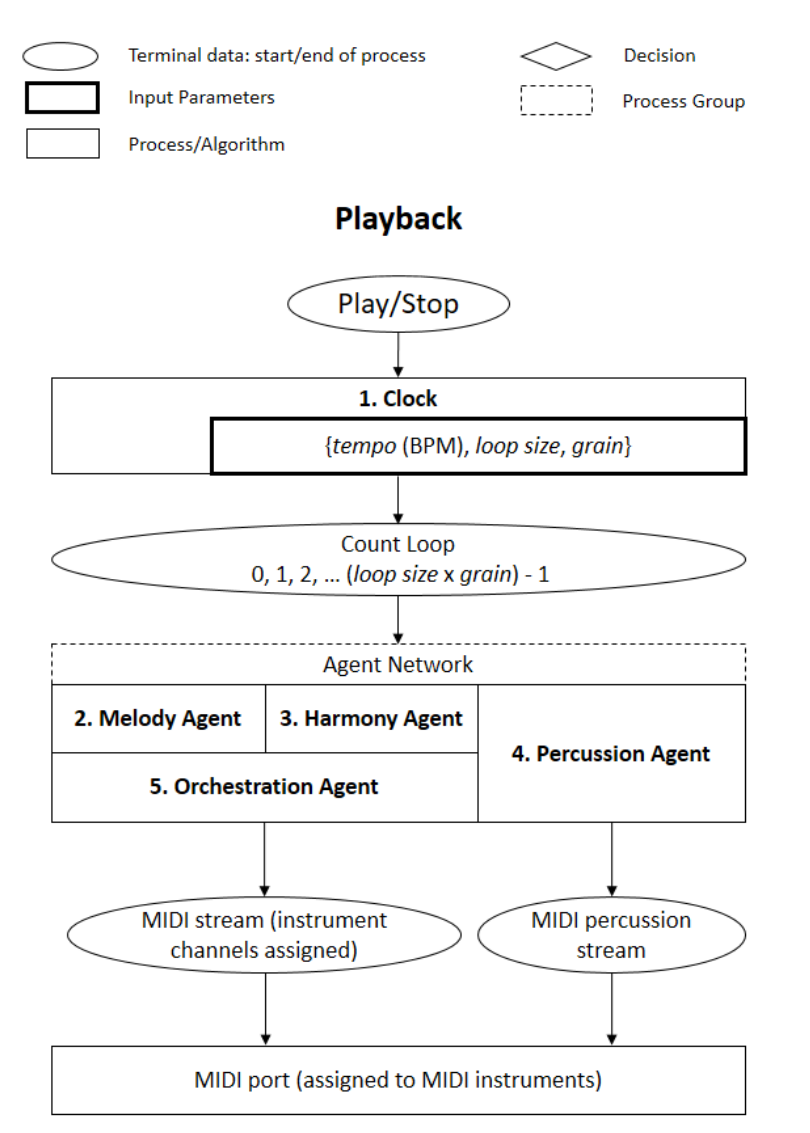
\includegraphics[width=\linewidth,height=10cm]{images/pamg_algorithm.png}
    \caption{Algorithm / architecture of PAMG \cite{lopez2023progressive}}
    \label{fig:pamg_algorithm}
\end{figure}


\subsubsection{Melody Agent}

The Melody Agent is responsible for generating melodies as outlined in previous sections \cite{lopez2023progressive}. Initially, the Melody Agent engages in rhythm generation by producing a list of onsets based on the beat, which is then manipulated to create syncopation. This process yields two lists: the Moved List and the Beat List \cite{lopez2023progressive}. Subsequently, the onsets are subject to stochastic modifications, either added or removed randomly from these lists \cite{lopez2023progressive}. The duration of each onset is then determined, classified as either staccato or legato \cite{lopez2023progressive}.

Following the completion of rhythm generation, the next step is velocity generation \cite{lopez2023progressive}. This involves employing a stochastic sequence to determine the MIDI velocity, or amplitude, for each onset, ultimately producing a MIDI velocity value for every onset \cite{lopez2023progressive}.

Pitch generation occurs after velocity determination \cite{lopez2023progressive}. This phase comprises three sub-processes: note stream generation, transposition, and harmony filtering \cite{lopez2023progressive}. The algorithm incorporates both "drunk" and "drunk-contour" modes for pitch generation, with each mode producing a pitch value that is subsequently adjusted through the transposition algorithm to refine the pitch \cite{lopez2023progressive}. A harmony filter is then applied to harmonize the pitch value \cite{lopez2023progressive}.

Once pitch generation is complete, the melody is developed through temporal transposition \cite{lopez2023progressive}. Subsequently, melody modification involves changing the transposition based on an analysis of previous pitches and generating new transposition values \cite{lopez2023progressive}. Additionally, phrase changes are implemented, altering rhythmic patterns according to harmonic structures \cite{lopez2023progressive}. These modifications are integrated into the MIDI event construction, resulting in a MIDI event stream that is forwarded to the Orchestration Agent \cite{lopez2023progressive}.

\subsubsection{Harmony Agent}

The Harmony Agent commences with the generation of harmony rhythm \cite{lopez2023progressive}. This involves operating an accent/beat follower to produce an interpolated list of rhythmic accents derived from the Moved List and Beat List \cite{lopez2023progressive}. A seeded random generator is used to introduce syncopation or adherence to beats \cite{lopez2023progressive}. Following this, the generated onsets are adjusted by adding or subtracting onsets based on harmony parameters \cite{lopez2023progressive}. A binary sequence for staccato/legato is then applied to determine the duration of each onset \cite{lopez2023progressive}.

After rhythm generation, the Harmony Agent progresses to velocity generation \cite{lopez2023progressive}. This step involves creating MIDI velocity values for chord onsets or arpeggio pitches, with a focus on onsets from the Moved List \cite{lopez2023progressive}.

The subsequent process is harmony sequence generation \cite{lopez2023progressive}. The module selects chord changes within a loop, ensuring that certain transitions are avoided at the beginning and end to facilitate longer resolutions \cite{lopez2023progressive}. It manages chord pools and their progression, determining the available chords and their sequence based on complexity \cite{lopez2023progressive}. Using a chord dictionary, pitch-class lists for chords are retrieved and adjusted for dissonance if required \cite{lopez2023progressive}. The chord builder then constructs pitch lists for playback, organizing intervals to emulate orchestration, while the arpeggiator generates arpeggio patterns based on orchestration settings and other parameters \cite{lopez2023progressive}.

Following the completion of harmony sequence generation, the harmony change algorithm prepares and implements changes to register and onset parameters, utilizing a random generator with constraints to prevent frequent modifications \cite{lopez2023progressive}. MIDI event construction then integrates all calculated outputs to produce a MIDI stream, which is forwarded to the Orchestration Agent \cite{lopez2023progressive}.


\subsubsection{Percussion Agent}

The Percussion Agent is responsible for generating rhythms for percussion instruments using various algorithms \cite{lopez2023progressive}. The Accent/Beat Follower interpolates syncopations for all percussion instruments based on the Moved List and Beat List \cite{lopez2023progressive}. The Additive and Subtractive Filling algorithm then allocates these onsets to different percussion instruments, such as kick/snare, toms, and cymbals, allowing for customizable patterns and offsets \cite{lopez2023progressive}.

Velocity generation determines the velocity parameter to set accents and produce MIDI velocity values \cite{lopez2023progressive}. The ratchet mechanism randomly selects the occurrence and type of ratchet (e.g., 64th, 32nd) for all instruments except the kick drum, calculating the corresponding velocity values \cite{lopez2023progressive}.

The percussion change function adjusts percussion parameters based on current chords to create variations. A random generator is used to determine changes that support the phrasing \cite{lopez2023progressive}.

In MIDI event construction, the Percussion Agent manages the pitch range of each instrument in MIDI pitch values and generates real-time MIDI events based on velocity, pitch, and a constant duration of 300 ms \cite{lopez2023progressive}. Non-zero values from the rhythm onset collection are used to trigger the generation of onsets, which are then formed into MIDI events \cite{lopez2023progressive}.

\subsubsection{Orcestration Agent}

The Orchestration Agent uses a random generator to manage the instrument families of the Melody/Harmony agents \cite{lopez2023progressive}. It adds or removes instruments for each agent by adjusting the Orch +/- parameters and distributes the instrument families to the Harmony Agent stream voices based on the Harmony Agent velocity (intensity when overlapping), voices and range parameters \cite{lopez2023progressive}. The instrument change occurs after two phrases without orchestration changes \cite{lopez2023progressive}. It sets the range for the Melody Agent's instrument voices using the Orch Range parameter and the Pitch Class List \cite{lopez2023progressive}. Flags are sent to the arpeggiator algorithm for solo brass and solo piano and receive arpeggiator on/off signals \cite{lopez2023progressive}. The instrument family range is managed via the pitch frame in MIDI pitch values (a non-real-time parameter) \cite{lopez2023progressive}. Finally, the agent sends the final MIDI events to the specified MIDI channels and ports \cite{lopez2023progressive}.
\section{Discussion and Comparison}

To discuss the effect and impact of adaptive and generative music on the player, three studies are first presented. The studies evaluate the subjective responses of the participants and compare these responses for environments with linear, adaptive or generative music.

\subsection{Study 1}
Hutchings and McCormack have adapted an AMS (adaptive music system) to the two video games "Zelda: Mystery of solarus" \cite{zeldamysteryofsolarus2011}  and "Starcraft ii: Wings of liberty" \cite{starcraftiiwingsofliberty} \cite{hutMcCormAms}. The system was integrated into the games so that it receives information about the current state of the game at runtime \cite{hutMcCormAms}. In addition, the musical output of the system was replaced with the output of the AMS \cite{hutMcCormAms}. 

The system was then evaluated in a study with 34 participants \cite{hutMcCormAms}. The participants were asked to provide information on their feeling of immersion, the quality of the music and the correlation between music and actions \cite{hutMcCormAms}. They were divided into two groups \cite{hutMcCormAms}. Group A plays the game "Zelda: Mystery of solarus" with original music and "Starcraft ii: Wings of liberty" with music from the AMS \cite{hutMcCormAms}. Group B runs through both games in the other environment \cite{hutMcCormAms}. This prevents a participant from playing one game in two different music environments and therefore reduces bias \cite{hutMcCormAms}.

Furthermore, during the evaluation, the participants were played a short section of music that represents a certain game state or is played at a certain point in the game \cite{hutMcCormAms}. The participants then had to assign a term for a concept from the game to this section of music that they thought best suit \cite{hutMcCormAms}. The four game concepts for the music sections are shown in Fig. \ref{fig:tutorial_gal_def}. Additional the accepted terms for every concept are listed. 
\begin{figure}
    \centering
    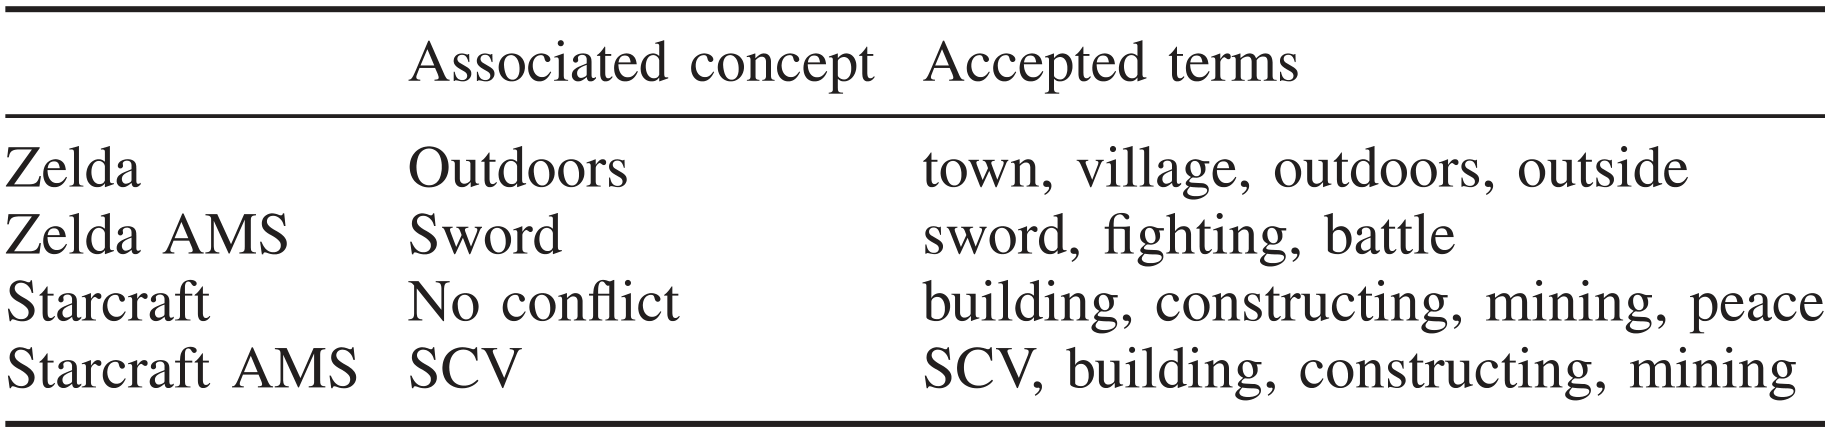
\includegraphics[width=1\linewidth]{images/ams_evaluation_table2.png}
    \caption{Accepted terms for established concepts \cite{hutMcCormAms}}
    \label{fig:ams_evaluation_table2}
\end{figure}
Participants of group A was played the music sections of the AMS conditions “Zelda AMS” and “Starcraft AMS” (see Fig. \ref{fig:tutorial_gal_def}) \cite{hutMcCormAms}. Group B was played the original music conditions “Zelda” and “Starcraft”) (see Fig. \ref{fig:tutorial_gal_def}) \cite{hutMcCormAms}.
For the “Zelda” condition, 70\% of participants stated a correct term. For the “Zelda AMS” condition, only 53\% of the participants reported one of the terms defined as correct \cite{hutMcCormAms}.
For music from the game “Starcraft ii: Wings of liberty” the results were similar with 59\% of participants assigning a correct term to the original music and 41\% of participants assigning a correct term to the music section of the AMS \cite{hutMcCormAms}.
This indicates that music from the AMS is more often misinterpreted and the associated game context is more likely to be confused than with the original, composed music.
However, the other reported results of the participants show a significant increase in the immersion and correlation of music and gameplay with the music output of the AMS compared to the original music \cite{hutMcCormAms}.

Hutchings and McCormack conclude that the AMS could be successfully applied to the games in this study \cite{hutMcCormAms}. Furthermore, they see the spreading activation model used for the AMS as a suitable model for analysing player emotions and game events \cite{hutMcCormAms}.

\subsection{Study 2}
Another study on the effects of adaptive music on the player was conducted by Plut and Pasquier \cite{plut2019music}. They created a video game called "Galactic Escape" using "FMOD Studio" \cite{fmod} to adapt the music to the gameplay \cite{plut2019music}. 25 participants took part in this study \cite{plut2019music}. Each participant played the game “Galactic defense” once with each of the four different music conditions (see Fig. \ref{fig:music_matters_table3}). The order of the music conditions was decided at random \cite{plut2019music}.
\begin{figure}
    \centering
    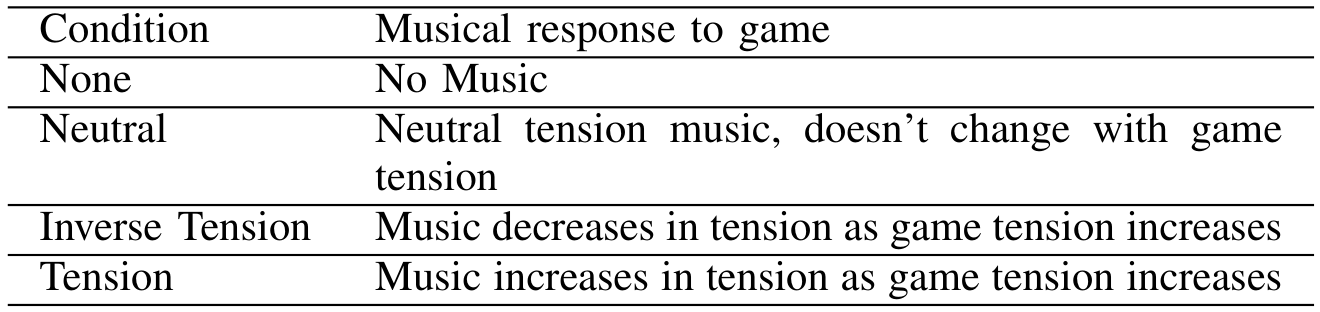
\includegraphics[width=1\linewidth]{images/music_matters_table3.png}
    \caption{Experimental conditions \cite{plut2019music}}
    \label{fig:music_matters_table3}
\end{figure}
After each game run, the participants report their enjoyment, affect and emotion by filling out a questionnaire \cite{plut2019music}. 

According to the results of the questions about enjoyment, the participants enjoyed the condition “None” (see Fig. \ref{fig:music_matters_table3}) without music the least \cite{plut2019music}. For the other three conditions the participants reported similar response values \cite{plut2019music}.

A greater difference between the conditions was reported for the perceived emotion \cite{plut2019music}. The participants indicate a higher response value for emotion in the "neutral" and "inverse tension" condition (see Fig. \ref{fig:music_matters_table3}) compared to the condition without music \cite{plut2019music}. For the "tension" condition, which features a congruent adaptation of music to the level of tension, the emotional response value is even higher than for the other conditions \cite{plut2019music}.

For the evaluation of the player's affect, Plut and Pasquier used a three-dimensional affect model with the dimensions valence, tension and arousal, which is a simplified version based on a more complex model by Schimmack and Grob \cite{schimmack2000dimensional} \cite{plut2019music}.
The questions about the player's affect are divided in one question for each dimension \cite{plut2019music}.
The response value for the dimensions arousal and valence show a similar trend and are similar to the emotional response (see Fig. \ref{fig:music_matters_experienced_affect}) \cite{plut2019music}. The arousal and valence value is higher for the "neutral" and "inverse tension" condition compared to the "none" condition without music \cite{plut2019music}. The values increase even further for the "tension" condition \cite{plut2019music}.
In contrast to this, the self-reported tension is decreased when music is introduced in the "neutral" condition compared to the "none" condition without music. However, it increases in the "inverse tension" and "tension" conditions, which feature adaptive music \cite{plut2019music}.
\begin{figure}
    \centering
    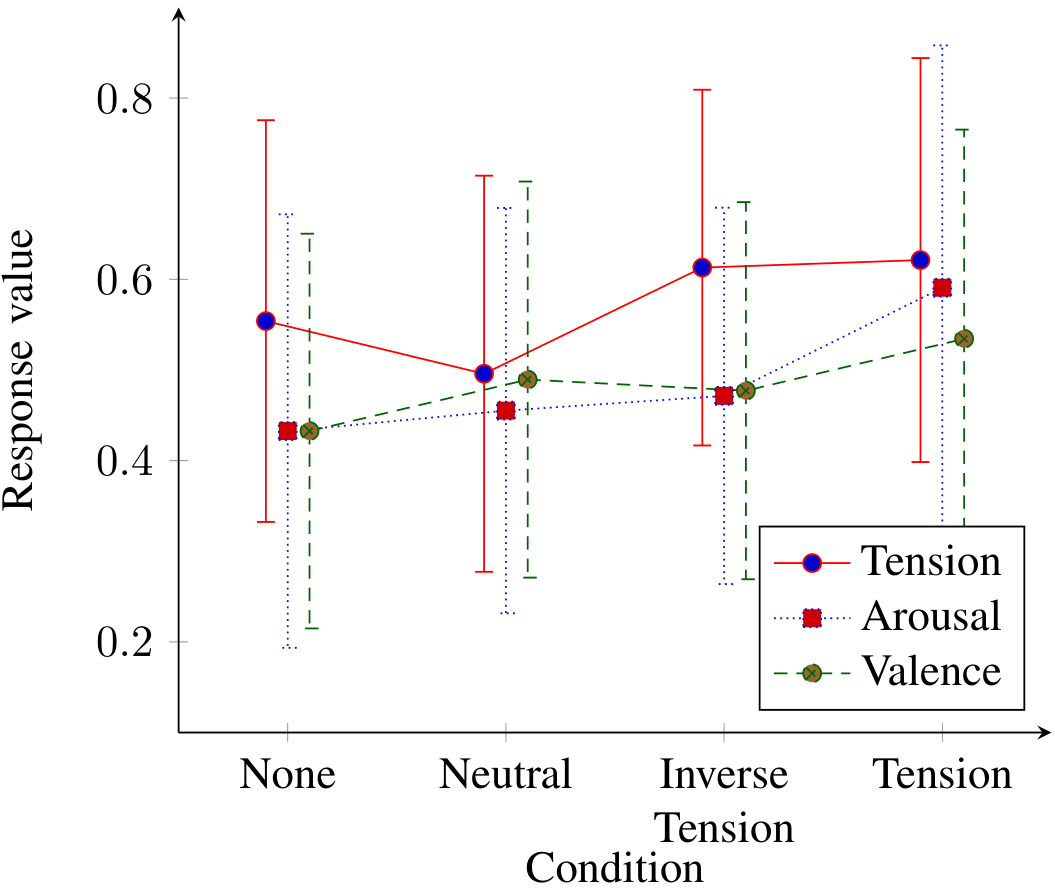
\includegraphics[width=1\linewidth]{images/music_matters_experienced_affect.png}
    \caption{Experienced affect means and Standard Deviations \cite{plut2019music}}
    \label{fig:music_matters_experienced_affect}
\end{figure}

The difference in self-reported tension between the "inverse tension" and "tension" conditions is minimal \cite{plut2019music}. This indicates that whether the music's tension adaptively matches the game's tension ("tension" condition) or is inversely adaptive to the game's tension ("inverse tension" condition), participants reported similar tension levels \cite{plut2019music}. Plut and Pasquier conclude from this that the adaptivity of the music is generally more important than the congruence between the game's tension and the music's tension \cite{plut2019music}. 
Furthermore they state, that "adaptive music increases player enjoyment, and
strengthens the affective impact of a game" \cite{plut2019music}. 


\subsection{Study 3}
In another study Plut et al. implemented different music scores into the video game "Galactiv Defense" \cite{plut2023preglam} \cite{plut2022preglam}. 
They created a linear, adaptive and generative musical score and integrated them into the game using the output of PreGLAM \cite{plut2023preglam} \cite{plut2022preglam}. 

To generate music for the generative score, the MMM model \cite{ens2020mmm} was used \cite{plut2022preglam}. Since the MMM model is not sufficiently efficient for real-time music generation, Plut et al. have pre-generated different music sections for different musical instruments. The compositions for the generative music are then randomly selected from the generated sections at runtime, ensuring a diverse and varied musical output \cite{plut2022preglam}.

To evaluate the various music scores, Plut et al. introduced 48 participants to the game through a tutorial, after which they could play the game freely \cite{plut2022preglam}. Additionally, each participant was shown four pre-recorded gameplay videos. Throughout the videos the participants reported their emotional responses \cite{plut2022preglam}. Finally, they matched each of four statements with the video they felt best represented it. The questions address the match between music and gameplay, the match between music and emotions, immersion and personal preference of music \cite{plut2022preglam}.

Overall, the study demonstrated that PreGLAM presents a effective emotion model for controlling adaptive music, as generative music provides improvements in emotional congruency and immersion compared to purely human-composed adaptive music \cite{plut2022preglam}.
Nevertheless, linear music received slightly higher ratings than generative music in the survey, but generative music was still generally rated better than composed adaptive music \cite{plut2022preglam}.
Plut et al. conclude that the linear score could be preferred over the generative score, as the linear score is the only one that contains specially composed transitions and could therefore be of higher quality than the other musical scores \cite{plut2022preglam}. 
They also state that the generative approach can offer much more musical diversity and can be less repetitive than composed music \cite{plut2022preglam}. 


\subsection{Evaluation of PAMG}
Lopez Duarte evaluated a generative and progressive adaptive music model PAMG in his dissertation \cite{lopez2023progressive}. The system was evaluated against an audio clip-based music (CBI) system using Wwise \cite{wwise} middleware \cite{lopez2023progressive}. The evaluation compared the PAMG and CBI models through a gameplay test with 18 participants \cite{lopez2023progressive}. The goal was to determine how the PAMG model impacts the gameplay experience compared to pre-recorded music in the CBI system \cite{lopez2023progressive}.

The participants were divided into two groups, “CBI first” and “PAMG first,” and played a video game created for the research \cite{lopez2023progressive}. Each group played the game twice, once with the PAMG system and once with the CBI system \cite{lopez2023progressive}. The “CBI first” group started with the CBI run, while the “PAMG first” group began with the PAMG system \cite{lopez2023progressive}.

Lopez Duarte concluded from the evaluation data that there were no statistically significant differences between the two models \cite{lopez2023progressive}. However, the results showed a slight preference for the PAMG model, with the generative and progressive-adaptive PAMG system receiving slightly higher overall ratings compared to the CBI system \cite{lopez2023progressive}.


\subsection{Comparison}
Adaptive and generative systems both create music based on game states, variables or other data from the video game \cite{plut2020generative} \cite{plut2022preglam}. The more these systems are integrated into a game, the more difficult it is to understand or predict the decisions made by the systems, as the increasing dependencies make the algorithms more complex. A resulting thesis is that adaptive and generative systems may face significant issues with consistency, reliability, and predictability.

As demonstrated by the survey in the third study presented \cite{plut2022preglam}, linear music may be preferred over adaptive or generative music. This study concludes that this could be due to a lack of explicitly composed transitions in the adaptive and generative music \cite{plut2022preglam}. Another reason for this result could be that linear music is preferred because it provides a deliberate and predefined emotional experience.

One conclusion from the first study \cite{hutMcCormAms} is that adaptive music can be misinterpreted more quickly in relation to the intended game context than the original hand-composed music. 

These results support the thesis that consistency and reliability are problematic for adaptive and generative music. Additionally, they suggest that the overall quality of music produced by these systems may be lower. Nevertheless, the evaluation results from the second study indicate that adaptive music can enhance player enjoyment and amplify the emotional impact of a game \cite{plut2019music}. 
This suggests that the primary advantage of adaptive and generative music over linear music lies in its ability to align more closely with the events and actions in the game. Rather than producing music of higher quality than hand-composed linear scores, adaptive and generative music is characterized by its ability to respond to the events and actions in the game.
In terms of quality, adaptive music systems may produce higher quality musical content than generative systems, as it uses hand-composed music sections \cite{plut2020generative}, which can individually have a higher quality.

Regarding the effects of adaptive and generative music on players in videogames, the studies show slight variations in their results but generally point in a similar direction. 
Compared to the original linear music of the games, the first study indicates a significant increase in immersion with adaptive music \cite{hutMcCormAms}. In the second study, participants reported increased enjoyment with adaptive music compared to linear music \cite{plut2019music}. The results of the third study show increased emotional congruence and enhanced immersion with generative music compared to linear or adaptive music \cite{plut2022preglam}. However, as shown in Fig. \ref{fig:preglamm_mmm_questionnaire_responses}, participants rated linear music slightly higher than generative music in the survey of this study. Nonetheless, generative music was rated overall higher than adaptive music \cite{plut2022preglam}.
\begin{figure}[h]
    \centering
    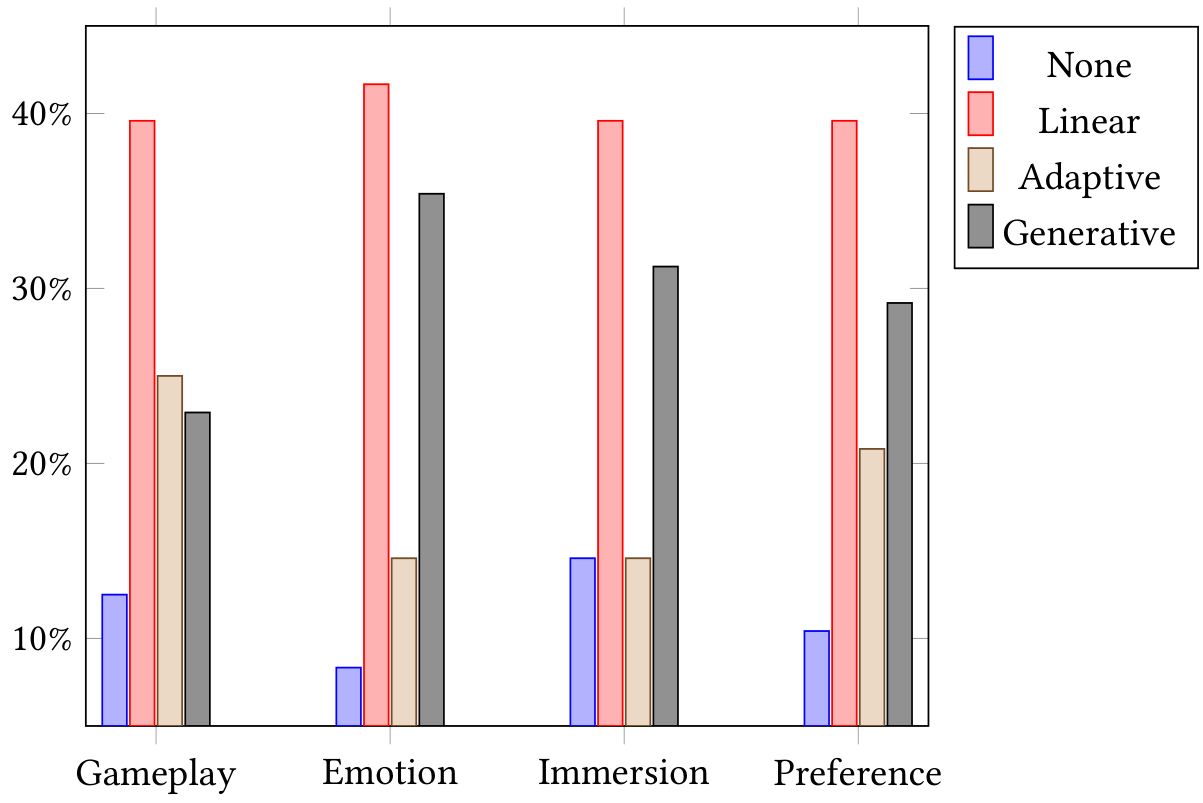
\includegraphics[width=1\linewidth]{images/preglamm_mmm_questionnaire_responses.png}
    \caption{Distribution of questionnaire responses \cite{plut2022preglam}}
    \label{fig:preglamm_mmm_questionnaire_responses}
\end{figure}
In addition, Plut et al. suggest that linear and adaptive music may feel repetitive after a certain time \cite{plut2022preglam}. This could lead to generative music being preferred more likely after several repetitions of game, as it offers new musical content.

\subsection{Limitations}
When comparing the results of the studies, it is important to note that while the generative score in the third study creates unique music customized to the gameplay, the system does not support real-time generation \cite{plut2022preglam}. Although Plut et al. believe, that the musical variety is not noticeably influenced for the participants of the study \cite{plut2022preglam}, the results could still have been affected by this factor. 

Considering the disadvantages and technical challenges, generative music systems like MMM \cite{ens2020mmm} can be highly resource-intensive and computationally demanding \cite{plut2022preglam}. Plut et al. had to pre-generate music for their evaluation because the model was too slow to generate music in real-time \cite{plut2022preglam}.

As previously mentioned, the consistency, predictability, and reliability of adaptive and generative music systems are often problematic when compared to the quality of hand-composed music. While adaptive music can generally be better controlled, it is still not entirely predictable due to the system's deep integration into the game and its dependency on numerous variables.

Another challenge in adaptive music is ensuring that individual musical sections meet the necessary musical requirements. Theoretically, these sections could be composed independently of one another. However, in order to allow for as many possible combinations of the sections, they are often created with similar characteristics, such as tempo or key \cite{plut2020generative}. This approach is showcased in the video game "Red Dead Redemption" \cite{reddeadredemption2010}, where different musical sections are composed in the same key and tempo to support smooth transitions \cite{plut2020generative}.
While this strategy ensures seamless transitions, it can also limit musical variety and diversity. If the sections are composed with distinct musical characteristics, it may increase the complexity of combining them and require more implementation effort.


\subsection{Impact}
When implemented effectively, both adaptive and generative music can significantly enhance how the players connect with and enjoy video games. This result from the scientific work presented could engage game developers to implement adaptive and generative systems in video games. 
Nevertheless, it can be said that generative scientific models, such as MMM \cite{ens2020mmm}, are not yet practically usable in real-time applications due to their high resource demands. This, on the other hand, could encourage other researchers to enhance existing generative music models and algorithms or to develop new, improved ones.
\section{Future work (Jonas)}
\begin{itemize}
\item Ansätze darstellen, wie das Thema in Zukunft weiterentwickelt wird
\item Einfluss auf zukünftige wissenschaftliche Entwicklungen bzw. andere Themenbereiche
\end{itemize}


\section{Conclusion}

In this paper, we have shown a set of adaptive and generative
music composition systems. There were systems like the AMS of Hutchings and McCormack
\cite{hutMcCormAms} or the Progressive-Adaptive Music Generator
of Lopez \cite{lopez2023progressive} that are hybrid, using 
adaptive and generative components in their systems. Next to both of those systems, we have shown approaches that utilize the Transformer architecture like the system of Amaral et al.
\cite{amaral2022adaptive} and the Multi-Track Music Machine by 
Ens and Pasquier \cite{ens2020mmm}. Some of them utilize an
emotion model like the AMS \cite{hutMcCormAms} and the approach
of Amaral et al. \cite{amaral2022adaptive}. Some of those
systems have been evaluated.

The evaluation studies on adaptive and generative music show how these technologies impact player experience. According to their results \cite{hutMcCormAms} \cite{plut2019music} \cite{plut2022preglam}, adaptive and generative music systems can increase the enjoyment, affect and immersion of video games by reacting to current game state and game variables. Generative music has the potential to enhance musical diversity and reduce the repetitive nature often associated with linear music. However, this has not yet been empirically evaluated in one of the studies presented.
Nevertheless, the results of the studies show that adaptive and generative music are overall less consistent and reliable in quality compared to hand-composed linear music. Additionally, generative music systems can be quite resource-intensive, which currently causes problems to integrate those systems into video games for real-time performance \cite{plut2022preglam}.


\bibliographystyle{IEEEtran}
\bibliography{references}

\vspace{12pt}

\end{document}


